\documentclass{beamer}

\usepackage[T2A]{fontenc}
\usepackage[utf8x]{inputenc}
\usepackage[english,bulgarian]{babel}
\usepackage{multirow}

\mode<presentation> {
	\usetheme{Berlin}
}

%\usebackgroundtemplate {
%	\includegraphics[width=370px, height=270px, trim=0 0 0 -80px]{background}
%}

\graphicspath{{../images/}}

\title{Реорганизация на данните и обработка на символни низове}
\subtitle{Статистическа обработка на данни с R}

\author{Пламен Петров и Тодор Балабанов}

\date{31.V.2020}

\institute[ЦО и ИИКТ към БАН] {
	Център за обучение \\
	Институт по информационни и комуникационни технологии \\ 
	Българската академия на науките \\
	\medskip
	\textit{p.petrov@iit.bas.bg todorb@iinf.bas.bg}
}

\addtobeamertemplate{navigation symbols}{}{
	\usebeamerfont{footline}
	\usebeamercolor[fg]{footline}
	\hspace{1em}
	\insertframenumber/\inserttotalframenumber
}

\begin{document}

\begin{frame}
	\titlepage
\end{frame}

\section*{Теми}
\begin{frame}[shrink]
	\frametitle{Съдържание}
	\tableofcontents
\end{frame}

\section{Обединяване на множества от данни}

\begin{frame}
\center \huge{Обединяване на множества от данни}
\end{frame}

\subsection{Множества с идентична структура}

\begin{frame}
\frametitle{Обединяване на множества от данни}
\begin{block}{Обединяване по редове}
ds1 <- cbind(TV=c($"$BNT$"$, $"$bTV$"$, $"$Nova$"$), Channel=c(1,2,3), Rating=c(0.1,0.3,0.2))

ds2 <- data.frame(TV=c($"$HBO$"$, $"$VH1$"$, $"$MTV$"$), Channel=c(4,5,6), Rating=c(0.4,0.5,0.6), stringsAsFactors=FALSE)

ds <- rbind(ds1, ds2)
\end{block}
\end{frame}

\begin{frame}
\frametitle{Работа с външни данни}
\begin{block}{USAID множество от данни}
setwd( $"$\textasciitilde /Desktop$"$ )

download.file(url=$"$https://github.com/TodorBalabanov/Statistical-Data-Processing-with-R/raw/master/data/aid.zip$"$, destfile=$"$aid.zip$"$)

unzip($"$aid.zip$"$, exdir=$"$./$"$)
\end{block}
\end{frame}

\begin{frame}
\frametitle{Обработка на множество файлове}
\begin{block}{Зареждане USAID данните в R}
library( stringr )

for(file in dir($"$./$"$, pattern = $"$\textbackslash\textbackslash .csv$"$)) \{

	name <- str\_sub(string=file, start=12, end=18)

	data <- read.table(file=file.path($"$.$"$, file), header=TRUE, sep=$"$,$"$, stringsAsFactors=FALSE)

	assign(x=name, value=data)
	
\}
\end{block}
\end{frame}

\subsection{Функция merge}

\begin{frame}
\frametitle{Обработка по ключ}
\begin{block}{Сливане на данни с merge}
head(merge(x=Aid\_90s, y=Aid\_00s, by.x=c($"$Country.Name$"$, $"$Program.Name$"$), by.y=c($"$Country.Name$"$, $"$Program.Name$"$)))
\end{block}

\begin{block}{Сливане на данни при data.table}
library( data.table )

dt90 <- data.table(Aid\_90s, key=c($"$Country.Name$"$, $"$Program.Name$"$))

dt00 <- data.table(Aid\_00s, key=c($"$Country.Name$"$, $"$Program.Name$"$))

dt0090 <- dt90[ dt00 ]
\end{block}
\end{frame}

\subsection{Функция join}

\begin{frame}
\frametitle{Подобрено бързодействие}
\begin{block}{Сливане на данни с join}
library(plyr)

head( join(x=Aid\_90s, y=Aid\_00s, by=c($"$Country.Name$"$, $"$Program.Name$"$) ))
\end{block}
\end{frame}

\subsection{Транспониране на данните}

\begin{frame}
\frametitle{Предварителна обработка}
\begin{block}{От колони към редове}
library( reshape2 )

melt00 <- melt(Aid\_00s, id.vars=c($"$Country.Name$"$, $"$Program.Name$"$), variable.name=$"$Year$"$, value.name=$"$Dollars$"$)

head(melt00, n=3)

library( scales )

melt00\$Year <- as.numeric(str\_sub(melt00\$Year, start=3, 6))

melt00\$Program.Name <- str\_sub(melt00\$Program.Name, start=1, end=10)

melt00 <- aggregate(Dollars \textasciitilde Program.Name + Year, data=melt00, sum, na.rm=TRUE)
\end{block}
\end{frame}

\begin{frame}
\frametitle{Визуализация}
\begin{block}{Последваща обработка}
library( ggplot2 )

library( useful )

ggplot(melt00, aes(x=Year, y=Dollars)) + geom\_line(aes(group=Program.Name)) + facet\_wrap(\textasciitilde  Program.Name) + scale\_x\_continuous(breaks=seq(from=2000, to=2009, by=2)) + theme(axis.text.x=element\_text(angle=90, vjust=1, hjust=0)) + scale\_y\_continuous(labels=multiple\_format(extra=dollar, multiple=$"$B$"$))
\end{block}
\end{frame}

\begin{frame}
\frametitle{Разход на пари по програми и години}
\begin{figure}[]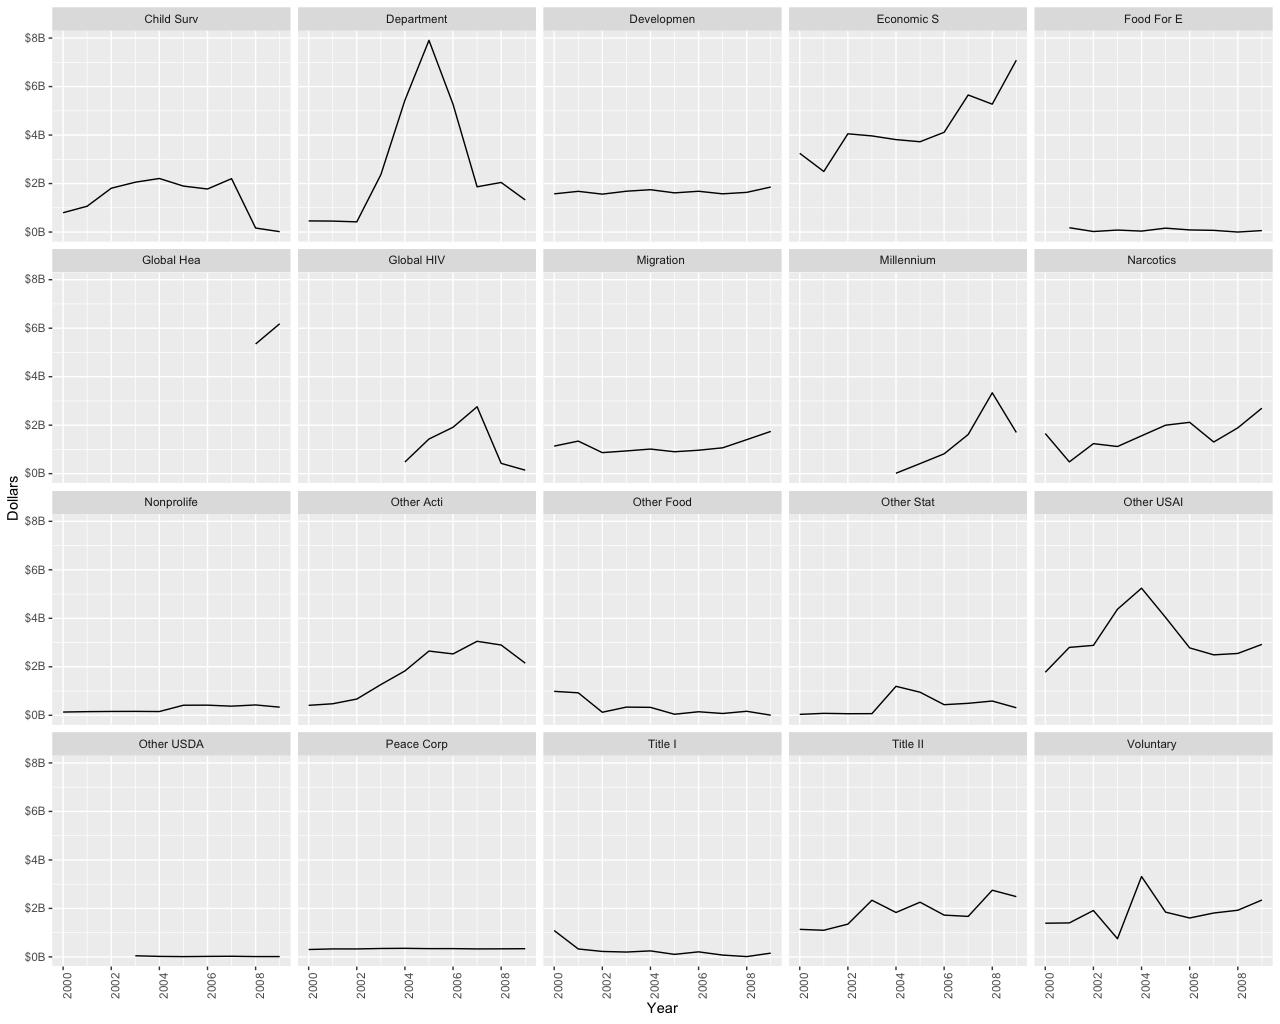
\includegraphics[width=\textwidth,height=0.75\textheight]{pic0029}\end{figure}
\end{frame}

\begin{frame}
\frametitle{Предварителна обработка}
\begin{block}{От редове към колони}
melt00 <- melt(Aid\_00s, id.vars=c($"$Country.Name$"$, $"$Program.Name$"$), variable.name=$"$Year$"$, value.name=$"$Dollars$"$)
 
cast00 <- dcast(melt00, Country.Name + Program.Name \textasciitilde Year, value.var=$"$Dollars$"$)
\end{block}
\end{frame}

\section{Сложни сливания на данни и трансформация на форматите}

\begin{frame}
\center \huge{Сложни сливания на данни и трансформация на форматите}
\end{frame}

\subsection{Обединение на редове и колони}

\begin{frame}
\frametitle{Разнородна организация на данните}
\begin{block}{Обединяване по колони и редове}
library(dplyr)

library(tibble)

ds1 <- bind\_cols(tibble(TV=c($"$BNT$"$, $"$bTV$"$, $"$Nova$"$), Channel=c($"$1$"$, $"$2$"$, $"$3$"$)), tibble(Rating=c($"$0.1$"$, $"$0.3$"$, $"$0.2$"$)))

ds2 <- tribble(\textasciitilde TV, \textasciitilde Channel, \textasciitilde Rating, $"$HBO$"$, $"$4$"$, $"$0.4$"$, $"$VH1$"$, $"$5$"$, $"$0.5$"$, $"$MTV$"$, $"$6$"$, $"$0.6$"$)

bind\_rows(ds1, ds2)
\end{block}
\end{frame}

\subsection{Сложни сливания на данни}

\begin{frame}
\frametitle{}
\begin{block}{Сложни сливания}
library( ggplot2 )

library( readr )

library( dplyr )

colors <- as\_tibble(read.table($"$https://raw.githubusercontent.com/TodorBalabanov/Statistical-Data-Processing-with-R/master/data/colors.csv$"$, header=TRUE, sep=$"$,$"$))

left\_join(diamonds, colors, by=c('color'='Color')) \%>\% select(carat, color, price, Description, Details)

tail(right\_join(diamonds, colors, by=c('color'='Color')))

inner\_join(diamonds, colors, by=c('color'='Color'))

semi\_join(colors, diamonds, by=c('Color'='color'))

anti\_join(colors, diamonds, by=c('Color'='color'))
\end{block}
\end{frame}

\subsection{Реформатиране на данните}

\begin{frame}
\frametitle{Зареждане на данни}
\begin{block}{Данни за реакциите}
library( readr )

emotions <- read\_tsv($"$https://raw.githubusercontent.com/TodorBalabanov/ Statistical-Data-Processing-with-R/master/data/reaction.txt$"$)
\end{block}
\end{frame}

\begin{frame}
\frametitle{Трансофрмации по колони и редове}
\begin{block}{Свиване от колони в редове}
library( tidyr )

emotions \%>\% gather(key=Type, value=Measurement, Age, BMI, React, Regulate)

gather(emotions, key=Type, value=Measurement, -ID, -Test, -Gender)
\end{block}
\end{frame}

\begin{frame}
\frametitle{Трансофрмации по колони и редове}
\begin{block}{Разпъване от редове в колони}
library( dplyr )

emotions \%>\% gather(key=Type, value=Measurement, Age, BMI, React, Regulate) \%>\% arrange(ID)

emotions \%>\% spread(key=Type, value=Measurement)
\end{block}
\end{frame}

\section{Работа със символни низове}

\begin{frame}
\center \huge{Работа със символни низове}
\end{frame}

\subsection{Формиране на текст}

\begin{frame}
\frametitle{Базови обработки}
\begin{block}{Конкатенация на символни низове}
paste($"$Hello$"$, $"$world$"$, $"$!$"$)

paste(c($"$Hello$"$, $"$world$"$, $"$!$"$), collapse=$"$ $"$)
\end{block}

\begin{block}{Печатане в текст}
name = $"$Todor$"$

sprintf($"$Hello, \%s!$"$, name)
\end{block}
\end{frame}

\subsection{Извличане на текст}

\begin{frame}
\frametitle{Обработка на неструктурирани документи}
\begin{block}{Достъп на HTML страници}
library( XML )

presidents <- readHTMLTable($"$http://www.loc.gov/rr/print/list/057\_chron.html$"$, which=3, as.data.frame=TRUE, skip.rows=1, header=TRUE, stringsAsFactors=FALSE)

library( stringr )

years <- str\_split(string=presidents\$YEAR, pattern=$"$-$"$)

ranges <- data.frame( Reduce(rbind, years) )

names( ranges ) <- c($"$Start$"$, $"$Stop$"$)
\end{block}
\end{frame}

\begin{frame}
\frametitle{Обработка на неструктурирани документи}
\begin{block}{Анализ на HTML страници}
presidents <- cbind(presidents, ranges)

presidents\$Start <- as.numeric( as.character(presidents\$Start) )

presidents\$Stop <- as.numeric( as.character(presidents\$Stop) )

presidents[str\_sub(string=presidents\$Start, start=4, end=4) == 1, c($"$YEAR$"$, $"$PRESIDENT$"$, $"$Start$"$, $"$Stop$"$)]
\end{block}
\end{frame}

\begin{frame}
\frametitle{Обработка по шаблон}
\begin{block}{Регулярни изрази}
presidents[ str\_detect(string=presidents\$PRESIDENT, pattern=$"$John$"$), c($"$YEAR$"$, $"$PRESIDENT$"$, $"$Start$"$, $"$Stop$"$) ]

sum( str\_detect(presidents\$PRESIDENT, $"$john$"$) )

sum( str\_detect(presidents\$PRESIDENT, ignore.case($"$John$"$)) )
\end{block}
\end{frame}

\begin{frame}
\frametitle{Обработка по шаблон}
\begin{block}{Сложни регулярни изрази}
conncetion <- $"$https://github.com/TodorBalabanov/Statistical-Data-Processing-with-R/raw/master/data/war.rdata$"$

load( conncetion )

close( connection )

wars[ str\_detect(string=wars, pattern=$"$-$"$) ]

str\_split(string=wars, pattern=$"$(ACAEA)|-$"$, n=2)
\end{block}
\end{frame}

\section{Заключение}

\begin{frame}
\center \huge{Заключение}
\end{frame}

\subsection{Дискусия}

\begin{frame}
\frametitle{Въпроси и отговори}
\center \huge{Благодаря за вниманието!}
\end{frame}

\end{document}
